\documentclass[twoside,11pt]{report}

% Any additional packages needed should be included after jmlr2e.
% Note that jmlr2e.sty includes epsfig, amssymb, natbib and graphicx,
% and defines many common macros, such as 'proof' and 'example'.
%
% It also sets the bibliographystyle to plainnat; for more information on
% natbib citation styles, see the natbib documentation, a copy of which
% is archived at http://www.jmlr.org/format/natbib.pdf

\usepackage{jmlr2e}
% \usepackage[utf8]{inputenc}%
% \usepackage{tikz}
% \usepackage{cfr-lm}%
\usepackage[T1]{fontenc}%
\usepackage{physics}
\usepackage{amsmath}
% \usepackage{amssymb}
% \usepackage{graphicx}
% \usepackage[margin=3cm]{geometry}
% \usepackage{changepage}
\usepackage{fontspec}
\usepackage{minted}
\usepackage{tcolorbox}
\usepackage{lmodern}
\usepackage{xcolor}
\usepackage{lettrine}
% \usepackage{fontawesome}
\usemintedstyle{perldoc}
\hypersetup{colorlinks=false, pdfborder={0 0 0},  }
\usepackage{fancyhdr}
\usepackage{wrapfig}
\usepackage{adjustbox}
\usepackage{tikz}
% \usepackage{listofitems} % for \readlist to create arrays
\usepackage{caption}
\usepackage[toc,page,header]{appendix}


\newtcbox{\codebox}[1][black]{on line, arc=2pt,colback=#1!10!white,colframe=white, before upper={\rule[-3pt]{0pt}{10pt}},boxrule=1pt, boxsep=0pt,left=2pt,right=2pt,top=1pt,bottom=.5pt}
\newtcbox{\deloppg}[1][black]{on line, arc=2pt,colback=#1!10!white,colframe=white, before upper={\rule[-2pt]{0pt}{0pt}},boxrule=0pt, boxsep=0pt,left=.49\linewidth,right=.49\linewidth,top=4pt,bottom=3pt}


\newcommand\blfootnote[1]{ \begingroup \renewcommand\thefootnote{}\footnote{#1} \addtocounter{footnote}{-1} \endgroup }
% \definecolor{antwhite}{HTML}{323333}
\newcommand{\code}[3][]{\codebox{\mintinline[#1]{#2}{#3}}}



% \setmainfont{FreeSans}
% \setmainfont{SF Pro Display}
% \setmainfont{IBM Plex Sans}
% \setmainfont{TeX Gyre Heros}
% \setmainfont{Inter}
% \setmainfont{Iosevka Quasi}
% \setmainfont{DM Sans}

% \setmonofont{Iosevka Custom Extended}
% \setmonofont{JetBrainsMono Nerd Font}
\setmonofont[Scale=MatchLowercase]{DM Mono}





% Definitions of handy macros can go here

\newcommand{\dataset}{{\cal D}}
\newcommand{\fracpartial}[2]{\frac{\partial #1}{\partial  #2}}

\newtcolorbox[blend into=tables]{mytable}[2][]{float=htb, halign=center,  title={#2}, every float=\centering, #1}
% Heading arguments are {volume}{year}{pages}{submitted}{published}{author-full-names}

% \jmlrheading{1}{2000}{1-48}{4/00}{10/00}{https://github.com/bragewiseth/MachineLearningProjects}

% Short headings should be running head and authors last names

\ShortHeadings{\url{https://github.com/bragewiseth/MachineLearningProjects}}{\url{https://github.com/bragewiseth/MachineLearningProjects}}
\firstpageno{1}



\title{{Solving the Wave Equation with Neural Networks}}
\author{\name Brage W. \email bragewi@ifi.uio.no\\
    \name Felix C. H.  \email felixch@ifi.uio.no \\
\name Eirik B. J. \email eiribja@ifi.uio.no}
\date{\today}											% Date
\makeatletter






% \date{\today}

\usepackage{hyperref}
\begin{document}

%%%%%%%%%%%%%%%%%%%%%%%%%%%%%%%%%%%%%%%%%%%%%%%%%%%%%%%%%%%%%%%%%%%%%%%%%%%%%%%%%%%%%%%%%

\begin{titlepage}
    \centering
    \vspace*{0.5 cm}
    
\includegraphics[scale = 0.70]{uio.jpg}\\[0.2 cm]	% University Logo
    \textsc{\LARGE University of Oslo}\\[2.0 cm]	    % University Name
    \textsc{\Large FYS-STK3155}\\[0.5 cm]				% Course Code
    \rule{\linewidth}{0.2 mm} \\[0.4 cm]
    { \huge \bfseries \@title}\\
    \rule{\linewidth}{0.2 mm} \\[1.5 cm]

    \begin{minipage}{0.4\textwidth}
        \begin{flushleft} \normalsize
            Brage Wiseth\\
            Felix Cameren Heyerdahl\\
            Eirik Bjørnson Jahr\\
        \end{flushleft}
    \end{minipage}~
    \begin{minipage}{0.4\textwidth}
        \begin{flushright} \normalsize
            \textsc{
                bragewi@ifi.uio.no\\
                felixch@ifi.uio.no\\
                eiribja@ifi.uio.no\\
            }
        \end{flushright}

    \end{minipage}\\[2 cm]
    \@date\\
    \vspace*{25mm}
    \urlstyle{rm}
    \textsc{\url{https://github.com/bragewiseth/MachineLearningProjects}}







\end{titlepage}
% \maketitle
\newpage
\tableofcontents
\newpage
\nocite{*}




\begin{abstract}%   <- trailing '%' for backward compatibility of .sty file
    \lettrine{T}{}his study explores the application of neural networks, specifically 
    Physics Informed Neural Networks (PINNs) 
    and Recurrent Neural Networks (RNNs), in solving the wave equation, contrasting their effectiveness 
    with classical methods like finite difference and analytical solutions. It demonstrates the feasibility
    of employing neural networks for solving partial differential equations (PDEs), offering a proof of 
    concept for future research in this domain. We found that neural networks are indeed capable of approximating
    the wave equation, although the accuracy of the models is not as high as we would have hoped. For our
    simple case where both analytical and finite difference solutions are available, the neural network
    models are not able to achieve the same accuracy. The PINN manages to capture the physical laws embedded
    in its loss function, but fails to generalize to other initial conditions. The RNN is able to capture
    the temporal dynamics of the wave equation, but fails to capture the spatial dynamics. The hybrid solver
    is able to capture both the spatial and temporal dynamics, but fails to generalize to other initial conditions.
    Although the neural nets indeed learn the dynamics of waves, they also suffer from artifacts, such as
    violating energy conservation.
    Despite this, our study demonstrates the potential of neural
    networks in solving more complex PDEs, paving the way for future research in this field.
\end{abstract}
\begin{keywords}
PINNs, RNNs, PDEs, Wave Equation, Neural Networks
\end{keywords}




\addcontentsline{toc}{section}{Introduction}
\section*{Introduction}

    Partial differential equations (PDEs) are ubiquitous in the field of physics and engineering,
    describing a wide range of phenomena, from fluid dynamics to quantum mechanics.
    PDEs are in a sense the language of physics, and as such, solving them yeilds valuable insights into
    the physical world. While analytical solutions are often preferred, they are not always feasible,
    they are often limited to simple cases with idealized boundary and initial conditions. Numerical methods, 
    although versatile, can be computationally 
    demanding and less accurate over time. In recent years, the advent 
    of deep learning has opened new avenues for addressing complex computational problems.
    The primary aim of this paper is to serve as a proof of concept for the use of neural networks in solving
    partial differential equations. As neural networks are universal function approximators, they should be 
    capable of approximating the solutions to PDEs. A naive approach to employing neural networks for solving
    PDEs can be to simply train a dense neural network with heaps of simulated data. Without any prior knowledge
    about the problem, this approach is unlikely to yield good results and will require a lot of data. 
    \cite{krishnapriyan2021characterizing} By giving the neural network some help and insight about the specific
    problem, we hope to drastically limit the search space of the neural network, and thus require less data.
    We will explore two different approaches to solving the wave equation with neural networks. The first approach
    is to use a Physics Informed Neural Network (PINN). PINNs are neural networks that incorporate physical laws
    into their loss function. This way the neural network can learn the underlying dynamics of the system, and
    thus require less data. The second approach is to use a Recurrent Neural Network (RNN). RNNs are neural networks
    that are able to process sequences. This way the neural network can learn the temporal dynamics of the system,
    and thus require less data. We will also explore a hybrid approach, where we use a finite difference scheme
    to generate data with labels, and use this data to define an error between the output of the neural network
    combined with physical laws. As previously mentioned, the primary aim of this paper is to serve as a proof
    of concept for the use of neural networks in solving partial differential equations. We will therefore
    not expoit the full potential of neural networks in this field.
    We leave the exploration and exploitation of the full potential of neural
    networks in this field to future work. 
    This research analyzes these neural network architectures, 
    discussing their theoretical frameworks, implementations, and comparative performance across accuracy, 
    efficiency, and scalability, thereby contributing to computational physics and engineering.

\section{Wave Equation}
\label{sec:wave}

    The wave equation, a fundamental partial differential equation, models wave propagation through 
    various media. It is mathematically represented as:
    \begin{equation}
    \frac{\partial^2 u}{\partial t^2} = c^2 \frac{\partial^2 u}{\partial x^2},
    \end{equation}
    where $u(x,t)$ denotes the displacement of the wave at position $x$ and time $t$, and $c$  
    signifies the wave speed. Typically, $x$ is considered within a 3-dimensional or 2-dimensional 
    space ($\mathbb{R}^3$ or $\mathbb{R}^2$) and $t$ within the temporal dimension ($\mathbb{R}$). 
    This paper, however, will focus on the one-dimensional spatial case ($x \in \mathbb{R}$).
    The equation illustrates that the wave's acceleration at a point in time is directly proportional to 
    its spatial curvature at that point. Solving the wave equation requires understanding the complex 
    interaction between its spatial and temporal aspects. While analytical solutions exist for certain 
    initial conditions, they are often impractical for more complex scenarios, necessitating the use of 
    numerical methods or neural networks.

\section{Data}
\label{sec:data}

    This study utilizes specific initial and boundary conditions to model the wave equation. 
    The initial conditions are set as follows:
    \begin{equation}
    u(x,0) = e^{-0.25x^2},
    \quad \frac{\partial u}{\partial t}(x,0) = 0,
    \end{equation}
    representing a Gaussian pulse with zero initial momentum at t=0t=0. 
    The boundary conditions are:
    \begin{equation}
    u(-5,t) = u(5,t) = 0.
    \end{equation}
    The analytical solution, derived from d'Alembert’s formula, serves as an accuracy benchmark for our methods:
    \begin{equation}
    u(x,t) = \frac{1}{2}(e^{-0.25(x+ct)^2} + e^{-0.25(x-ct)^2}).
    \end{equation}

    For the supervised and unsupervised learning approaches, we require labeled and unlabeled data, 
    respectively. In the supervised case (hybrid PINN), data is generated through a finite difference scheme. 
    In contrast, the unsupervised approach (plain PINN) relies on the network itself to generate labels.

    \subsubsection{Unsupervised Data}
    In unsupervised learning, we input coordinates $(x,t)$ and predict displacement $u(x,t)$ using 
    a uniform distribution for xx and tt. The "labels" are described by the wave equation.

    \subsubsection{Supervised Data}
    For supervised learning, we similarly input coordinates $(x,t)$, but the data is generated via a finite 
    difference solver. The loss function here compares the network output with the solver output.

    \subsubsection{Sequential Supervised Data (RNN)}
    for the RNN we input a sequence of spatial poitns at each time slice $\mathbf{x}_1, \mathbf{x}_2, \dots, \mathbf{x}_n$ 
    where $t_1, t_2, \dots, t_n$ are the time slices. The network then outputs the displacement at each of these points
    at each time slice. The loss function is then defined as the mean squared error between the output of the network
    if the input is the sequence of spatial points up to time $t_i$, the output of the network is the displacement
    at time $t_{i+1}$
    

\section{Methods}
\label{sec:methods}

    In this section we will describe the methods we have used to solve the wave equation.
    Some of the specific goals that each method aims to achieve differ, but they all aim to
    approximate the solution to the wave equation. We will start by describing the methods




\subsection{Finite Difference Scheme}
\label{sec:finite}

    A finite difference scheme is a numerical method for approximating the solutions to differential equations.
    The idea is to approximate the derivatives in the differential equation with finite differences.
    The simplest way to do this is to use the forward difference approximation:
    \begin{equation}
    \frac{\partial u}{\partial x} \approx \frac{u(x+h) - u(x)}{h}
    \end{equation}
    \begin{equation}
    \frac{\partial^2 u}{\partial x^2} \approx \frac{u(x+h) - 2u(x) + u(x-h)}{h^2}
    \end{equation}
    where $h$ is a small number. The smaller $h$ is, the more accurate the approximation will be.
    However, if $h$ is too small, the approximation will be unstable. The optimal value of $h$ depends
    on the problem. In our experiments we have used $h=0.01$.
    We can use the forward difference approximation to approximate the derivatives in the wave equation:
    \begin{equation}
    \frac{\partial^2 u}{\partial t^2} \approx \frac{u(x,t+h) - 2u(x,t) + u(x,t-h)}{h^2}
    \end{equation}
    \begin{equation}
    \frac{\partial^2 u}{\partial x^2} \approx \frac{u(x+h,t) - 2u(x,t) + u(x-h,t)}{h^2}
    \end{equation}
    We can then use these approximations to approximate the wave equation:
    \begin{equation}
    \frac{u(x,t+h) - 2u(x,t) + u(x,t-h)}{h^2} = c^2 \frac{u(x+h,t) - 2u(x,t) + u(x-h,t)}{h^2}
    \end{equation}
    We can then solve for $u(x,t+h)$:
    \begin{equation}
    u(x,t+h) = 2u(x,t) - u(x,t-h) + c^2(u(x+h,t) - 2u(x,t) + u(x-h,t))
    \end{equation}
    This is expression translates directly into code. We can use this to get a numerical solution to the wave equation.
    For each time step, the approximation gets more and more inaccurate. This is because the approximation is based on
    the previous time step, which is based on the time step before that, and so on. This way the error accumulates
    over time. For simulations that run for a long time, the error can become very large. One way to address this
    is to use a smaller time step $h$. Or as we propose in this paper, we can use a neural network to correct the
    error.


\subsection{Physics Informed Neural Networks (PINNs)}
\label{sec:DNN}
    
    The architecture is dense feed forward nn
    Physics Informed Neural Networks (PINNs) leverage the Universal Approximation Theorem, which posits 
    that a neural network with even a single hidden layer can approximate any function to a desired degree 
    of precision. This foundational principle enables neural networks to approximate complex functions, including 
    solutions to differential equations.
    PINNs, in particular, incorporate physical laws into their structure, allowing them to learn the underlying 
    dynamics of a system. For our case we wish to embed the wave equation into the loss function of the neural network.

    Generally, partial differential equations (PDEs) can be expressed in the form:
    \begin{equation}
    \resizebox{1.0\textwidth}{!}{$
        f\left(x_1, \, \dots \, , x_N, \frac{\partial g(x_1,\dots,x_N) }{\partial x_1}, 
            \dots , \frac{\partial g(x_1,\dots,x_N) }{\partial x_N}, \frac{\partial g(x_1,\dots,x_N) }
        {\partial x_1\partial x_2}, \, \dots \, , \frac{\partial^n g(x_1,\dots,x_N) }
        {\partial x_N^n} \right) = 0$
    }
    \end{equation}
    where $g(x_1,\dots,x_N)$ is the solution to the PDE. By expressing the PDE in this form, we can 
    see that the PDE is satisfied when $f=0$. We can then use this to define a loss function for the neural network:
    \begin{equation}
    \min_{P} \mathcal{L} = \min_{P} \sum_{i=1}^{N} f(x_i, P)
    \end{equation}
    where $P$ are the parameters of the neural network, and $x_i$ are the data points. 
    The specific form of $f$ for our case is:
    \begin{equation}
    f(x,t,P) = \frac{\partial^2 u}{\partial t^2} - c^2 \frac{\partial^2 u}{\partial x^2}
    \end{equation}
    where $u(x,t,P)$ is the solution to the wave equation. 
    In addition to minimizing eq. 13, we also want to ensure that the neural network satisfies the 
    initial and boundary conditions. We can propose a trial solution that ensures this:
    \begin{equation}
    u(x, t) = h_1(x, t) + h_2(x, t, N(x, t, P)),
    \end{equation}
    Here, $h_1(x,t)$ represents the initial and boundary conditions,
    while $h_2(x,t, N(x,t,P))$ ensures that the the output of the neural network respects 
    the initial and boundary conditions.
    The network minimizes the wave equation's residual, aligning the trial solution with the wave's true dynamics.
    In our specific implementation, we simply add the pure wave equation loss with the boundary and initial conditions loss.
    where the wave equation loss is the mean of eq. 13 over the data points, the initial conditions and boundary loss
    is defined as
    \begin{equation}
        u(x, 0) - \Omega  + \frac{\partial u}{\partial t}(x, 0) - \Gamma
    \end{equation}
    where $\Omega$ and $\Gamma$ are the initial conditions
    giving us the final loss function
    \begin{equation}
        \mathcal{L} = \frac{1}{N}\sum_{i=1}^{N} f(x_i, t_i, P) + u(x_i, 0) - \Omega  + 
        \frac{\partial u}{\partial t}(x_i, 0) - \Gamma
    \end{equation}
    \cite{fys-stk}
    \cite{krishnapriyan2021characterizing}



\subsection{Hybrid solver}
\label{sec:hybrid}
     
    As we have great control over the loss function, we can use this to our advantage. In some cases, a finite difference
    scheme may be quick to compute, and provide a decent approximation to the solution. We propose a hybrid solver, where
    we use a finite difference scheme to generate data with labels, and use this data to define an error between the
    output of the neural network and the finite difference scheme. We could in therory stop there and use this error
    as the loss function, however this will only give us a solution that is as good as the finite difference scheme.
    To improve on this, we can also add the wave equation as a constraint to the loss function.
    It is also possible to weight the components of the loss function differently, to give more or less 
    importance to the different components. We present an example of this in the implementation section.
    \begin{equation}
    \mathcal{L} = \alpha\mathcal{L}_{\text{FD}} + \mathcal{L}_{\text{PINN}}
    \end{equation}
    where $\mathcal{L}_{\text{FD}}$ is the loss from the finite difference scheme (or your favorite solver), 
    and $\mathcal{L}_{\text{PINN}}$ is the physics informed neural network loss. $\alpha$ is a hyperparameter
    that determines the relative importance of the two components of the loss function.
    \cite{krishnapriyan2021characterizing}

\subsection{Recurrent Neural Networks (RNNs)}
\label{sec:rnn}

    I problem with our current approch with PINNs is that we have to hard code the wave equation and the initial
    conditions into the loss function. This means that we have to train a new model for each set of initial conditions.
    In addressing the challenges posed by this lack of generalization, we can use a Recurrent Neural Network (RNN)
    to capture the temporal dynamics of the wave equation. This way we can train a single model that can be used
    to predict the evolution of the wave for any set of initial conditions. RNNs are distinguished by their ability to 
    process sequences and their inherent memory, making them well-suited for time-dependent problems.
    Our RNN model utilizes a series of LSTM (Long Short-Term Memory) layers, chosen for their 
    effectiveness in capturing long-range dependencies and mitigating the vanishing gradient problem.
    The network architecture is tailored to map the sequential nature of the wave data, taking 
    into account both spatial and temporal aspects.

    2. Data Preparation and Input Format:

        The input to the RNN is structured as sequences representing the state of the wave at consecutive 
        time steps.
        Prior to training, the data is preprocessed to normalize the amplitude of the wave, ensuring 
        consistent input value ranges for the network.

    When Not to Shuffle the Data

        Temporal Dependency: For problems where the goal is to predict future 
        states based on past states (like time series forecasting), the temporal 
        order of the data is crucial. The RNN learns to understand the sequence of 
        events or states, and shuffling would disrupt this order and potentially render 
        the data meaningless for the task.

        Sequential Learning: If each data point in your sequence depends on the previous 
        points (as is common in solving differential equations like the wave equation), 
        then maintaining the correct order of these points is essential for the model to 
        learn the underlying dynamics correctly.
        \cite{hu2022neuralpde}

    % \begin{figure}[!h]
    %     \begin{center}
    %         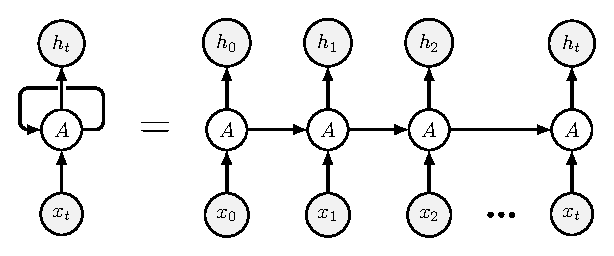
\includegraphics[width=0.8\textwidth]{tikzfigures/rnn.pdf}
    %     \end{center}
    %     \caption{A model of a neural network with one hidden layer consisting of four nodes}\label{fig:rnn}
    %     \cite{neutelings_tikzcode}
    % \end{figure}

\section{Results and Analysis}
\label{sec:resultsdiscussion}

\begin{mytable}[float=!h,label=tab:toyscores, width=0.5\textwidth]{Mean square error between analytical solution and different solvers.}
\centering
\begin{tabular}{l|l}
    Finite difference   &\texttt{0.00855}  \\
    PINN                &\texttt{0.879}  \\
    Hybrid              &\texttt{0.02}  \\
    Degree              &\texttt{0.02}  \\ 
\end{tabular}%
\end{mytable}
    
    loss function
    failures
    rescources
    time to train

    The way we implemented PINNs does not allow for genralization to other problems. This is because we have
    hard coded the wave equation and the initial conditions into the loss function. We also only have trainig data 
    for one set of initial conditions. However, 
    it may be possible to generalize the PINN 
    to other problems by using a more general loss function.
    When solving the wave equation with PINN overfitting in the traditional sense is not a problem, as the network
    aims to find an exact solution to the wave equation and not a general solution. With the hybrid solver and RNN
    however, overfitting  can pose a problem, and must be considered. For the hybrid solver, we can as mentioned
    weigh the components of the loss function differently to give more or less importance to the different components.
    and thus hinder overfitting. classical regularization techniques can also be used to prevent overfitting.



    Where the differnet features have vasly different scales, it might be a good idea to consider normalizing the data.
    however as our exmaple has featers with similar scales, we have not done this in our experiments.

    We used two hidden layers with 20 nodes each. We used the Adam optimizer with a learning rate of 0.01.

    The RNN takes significantly longer to train than the other models. This is because the RNN has to process
    the data sequentially, while the other models can process the data in parallel. The RNN also has to process
    the data in order, while the other models can process the data in any order. This means that the RNN has to


    \begin{figure}[!ht]
        \begin{minipage}[t]{0.5\textwidth - 1mm}
            \begin{center}
                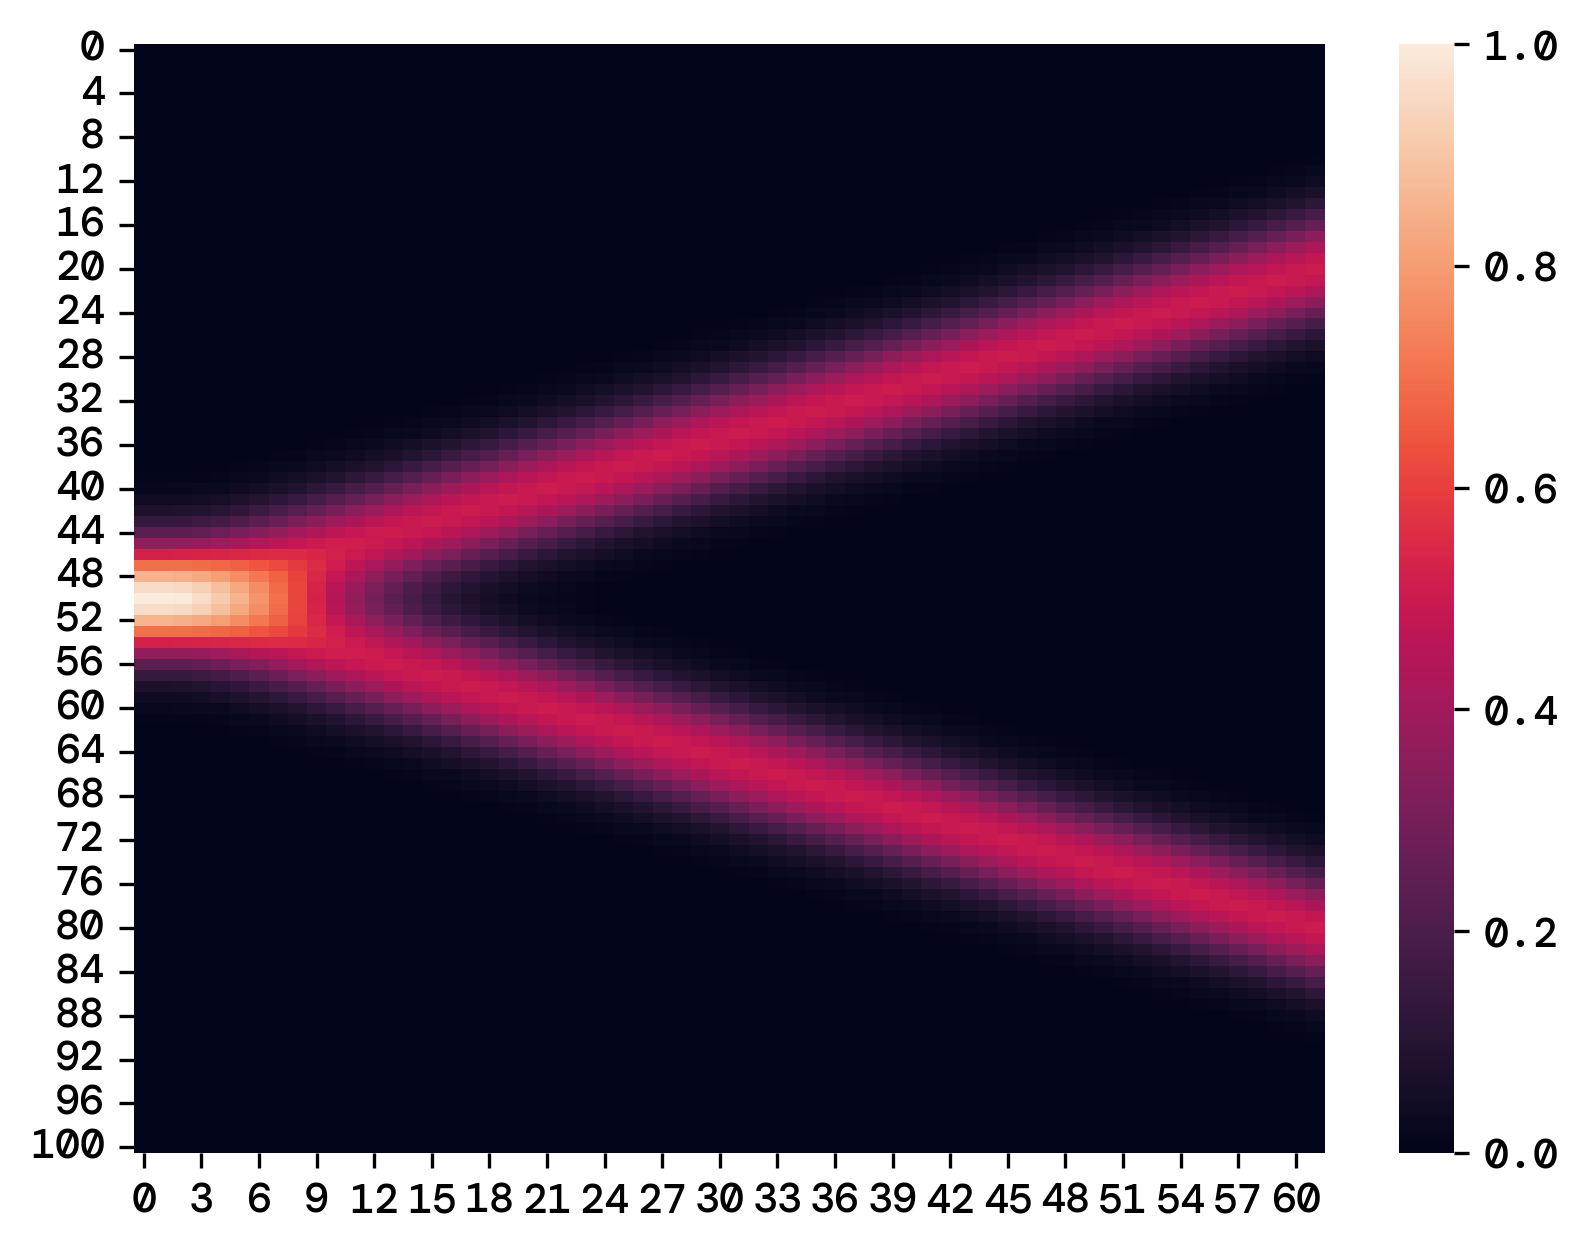
\includegraphics[width=\textwidth]{../runsAndFigures/wave_analytic.png}
            \end{center}
            \caption
            {
                Analytical solution to the wave equation.
            }\label{fig:wave_finite}
        \end{minipage}
        \hspace{2mm}
        \begin{minipage}[t]{0.5\textwidth - 1mm}
            \begin{center}
                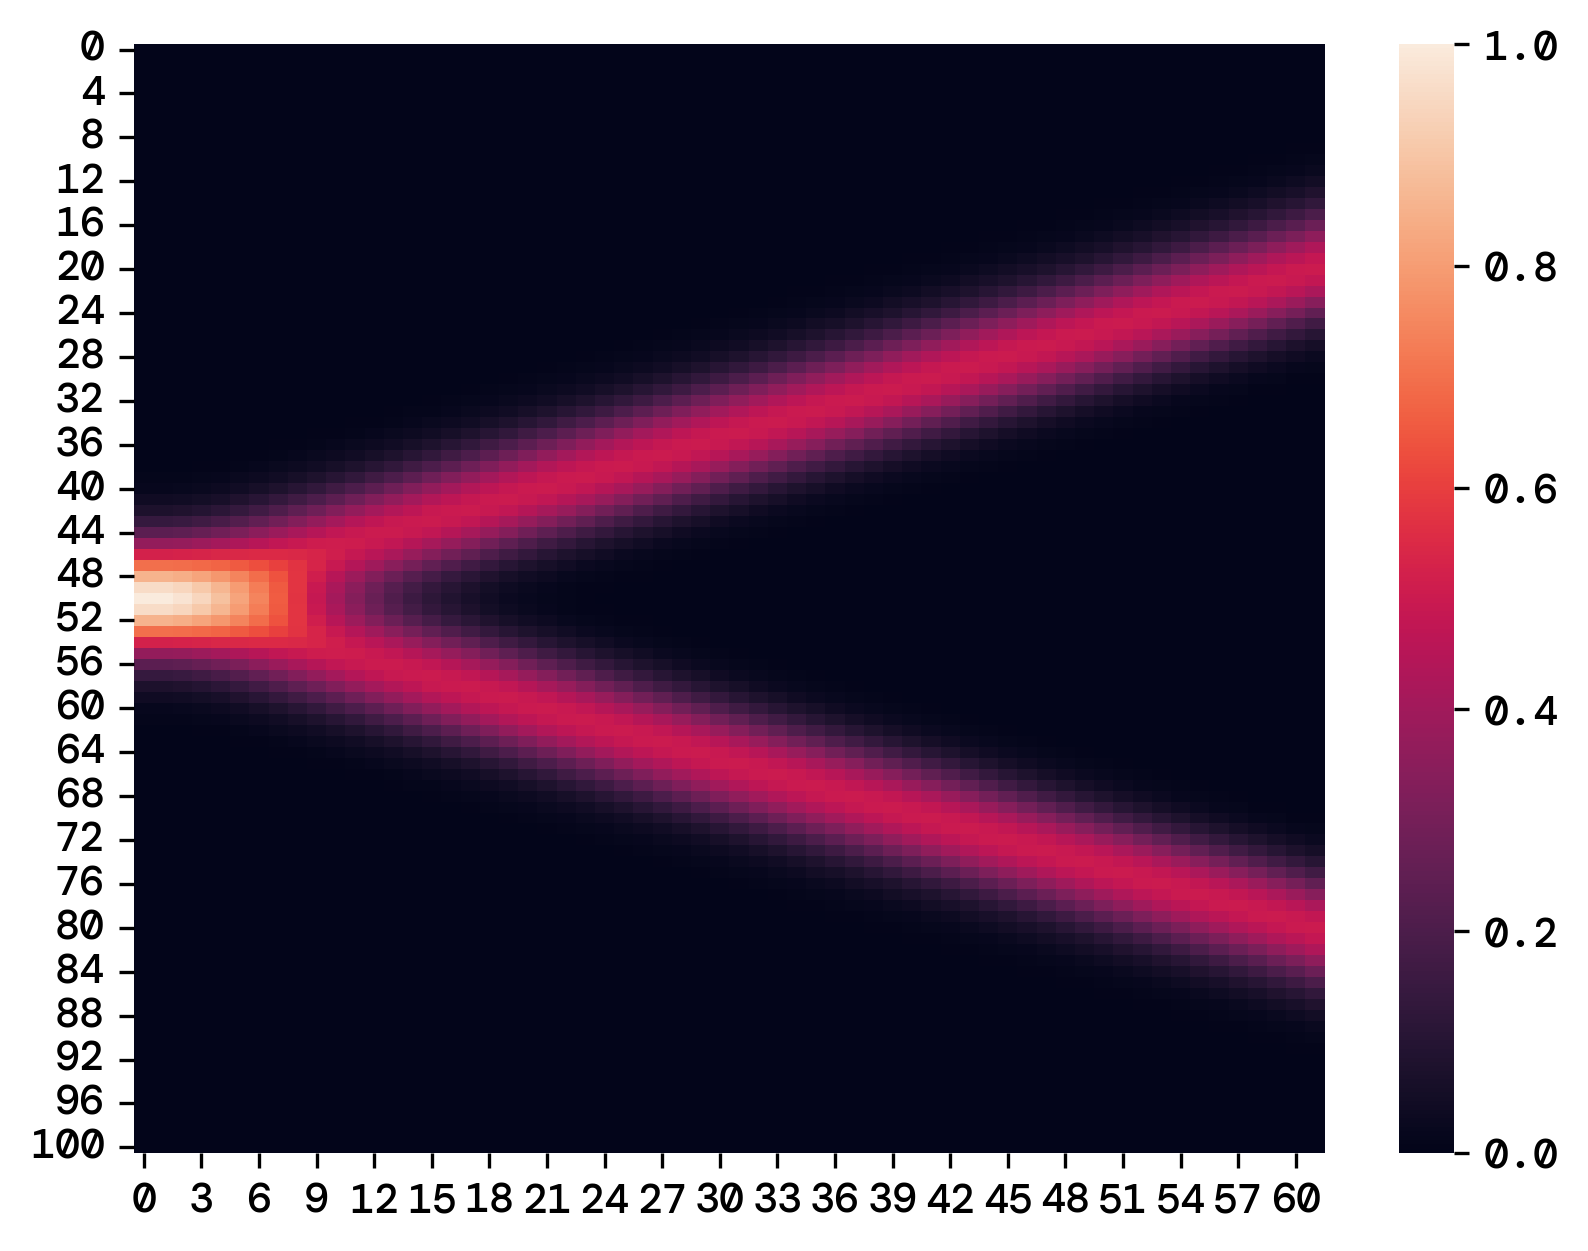
\includegraphics[width=\textwidth]{../runsAndFigures/wave_finite.png}
            \end{center}
            \caption
            {
                Finite difference solution to the wave equation.
            }\label{fig:wave_analytic}
        \end{minipage}
    \end{figure}
    \begin{figure}[!ht]
            \begin{center}
                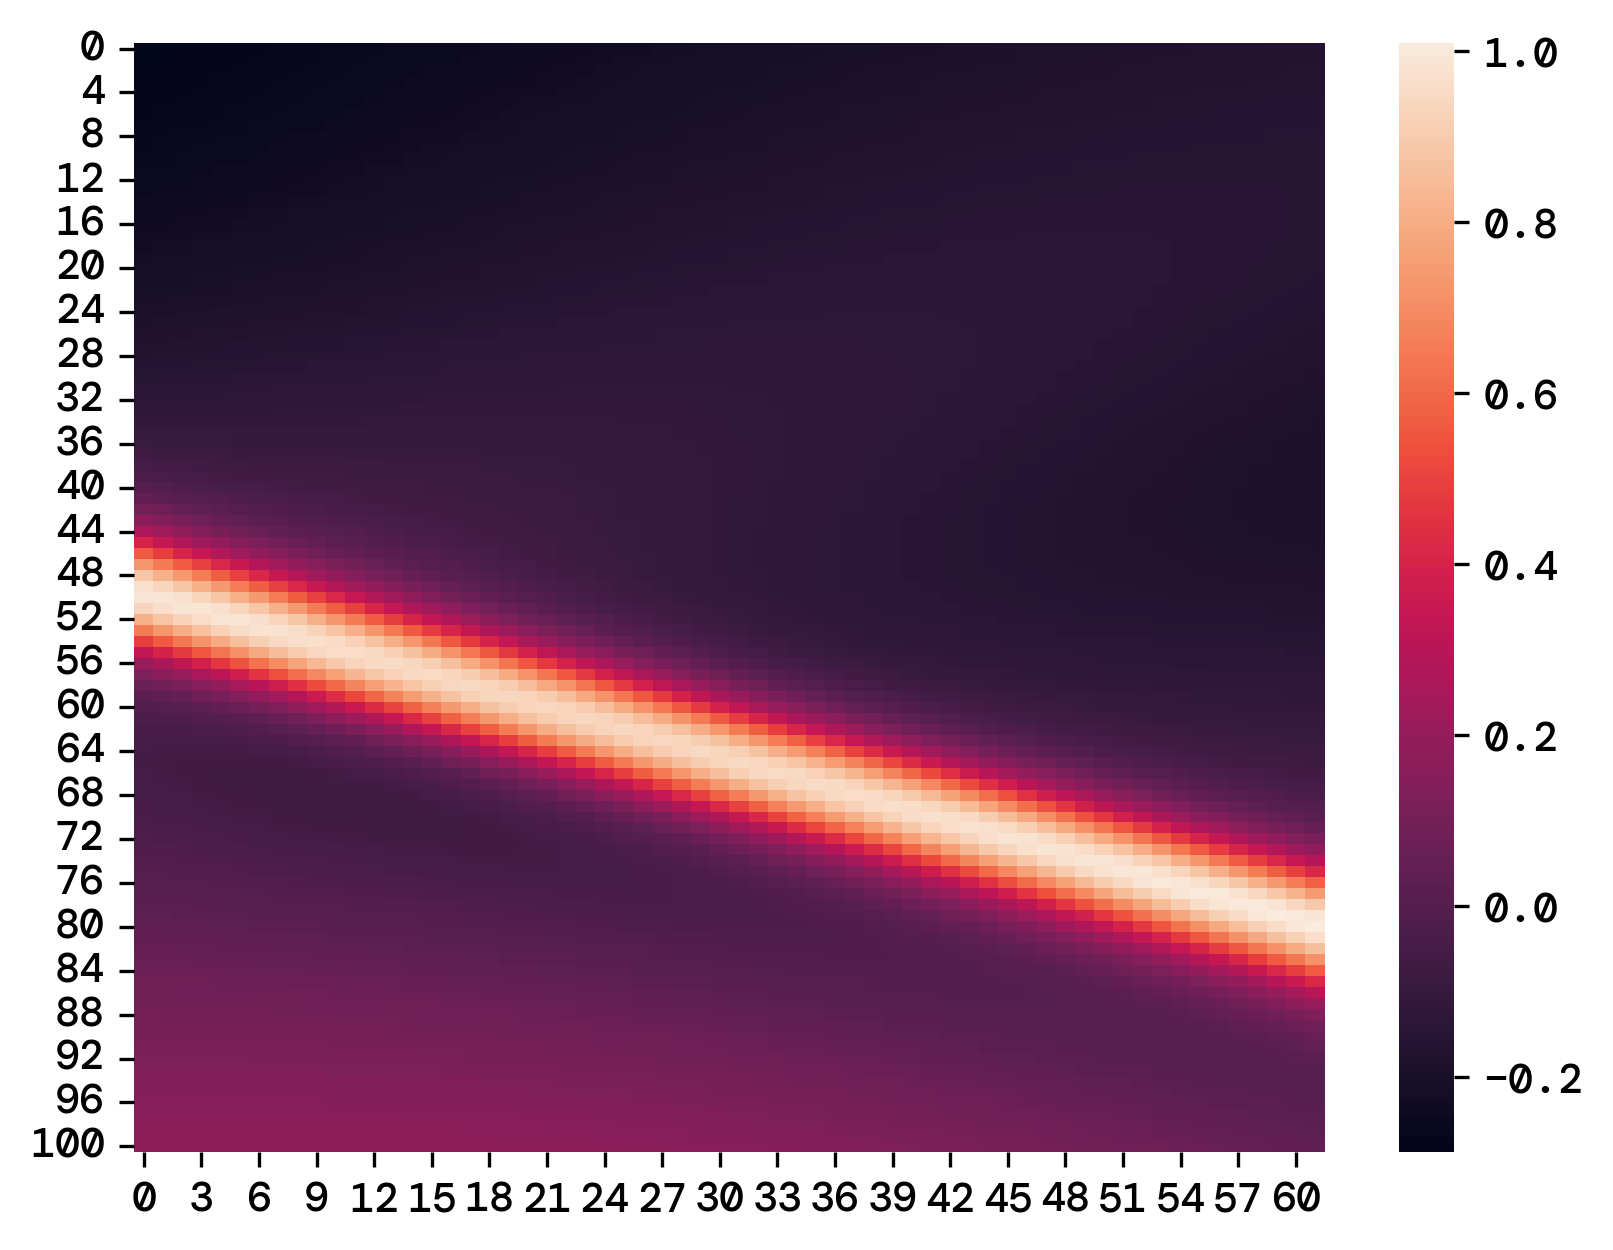
\includegraphics[width=0.5\textwidth]{../runsAndFigures/wave_tf_pinn_velocity.png}
            \end{center}
            \caption
            {
                The PINN learns a solution to the wave equation where the initial momentum is not defined.
                Yet it satisfies the wave equation and the initial conditions.
            }\label{fig:wave_tf_dnn}
    \end{figure}

    \begin{figure}[!ht]
        \begin{minipage}[t]{0.5\textwidth - 1mm}
            \begin{center}
                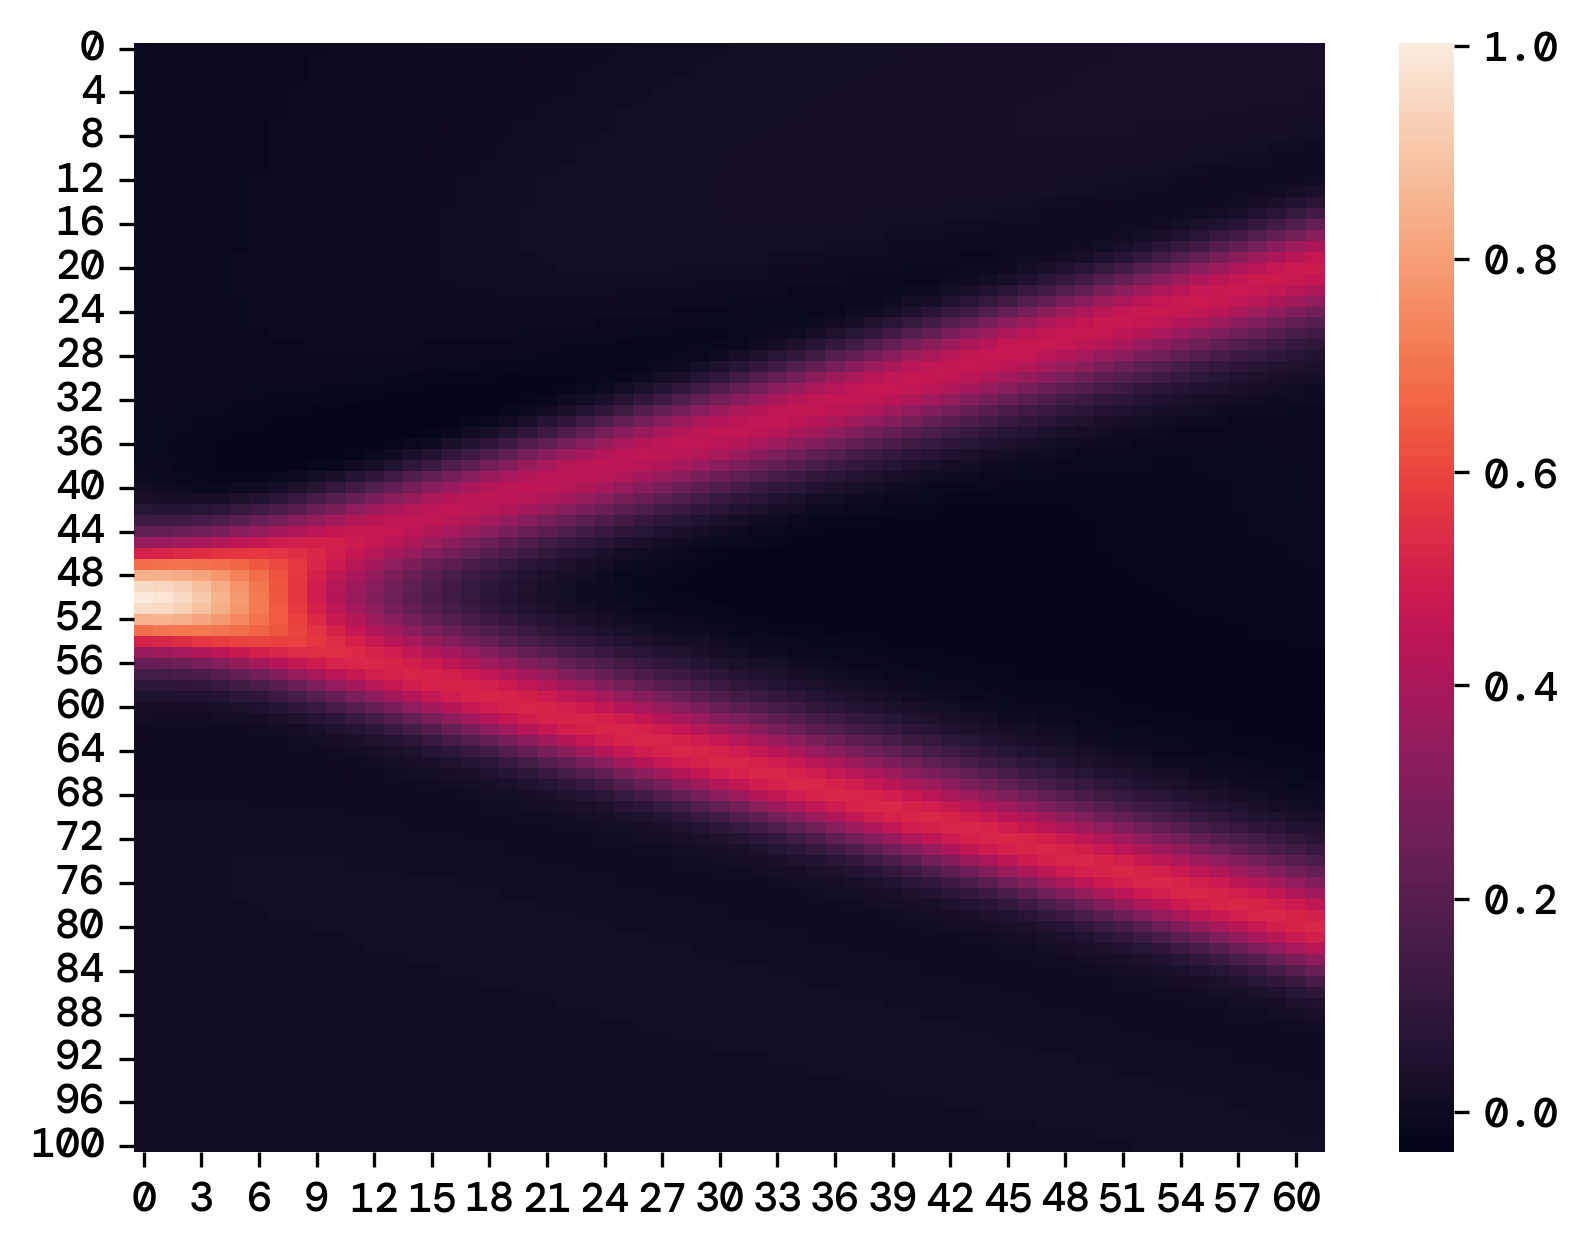
\includegraphics[width=\textwidth]{../runsAndFigures/wave_tf_hybrid.png}
            \end{center}
            \caption
            {
                PINN solution to the wave equation.
            }\label{fig:wave_own_dnn}
        \end{minipage}
        \hspace{2mm}
        \begin{minipage}[t]{0.5\textwidth - 1mm}
            \begin{center}
                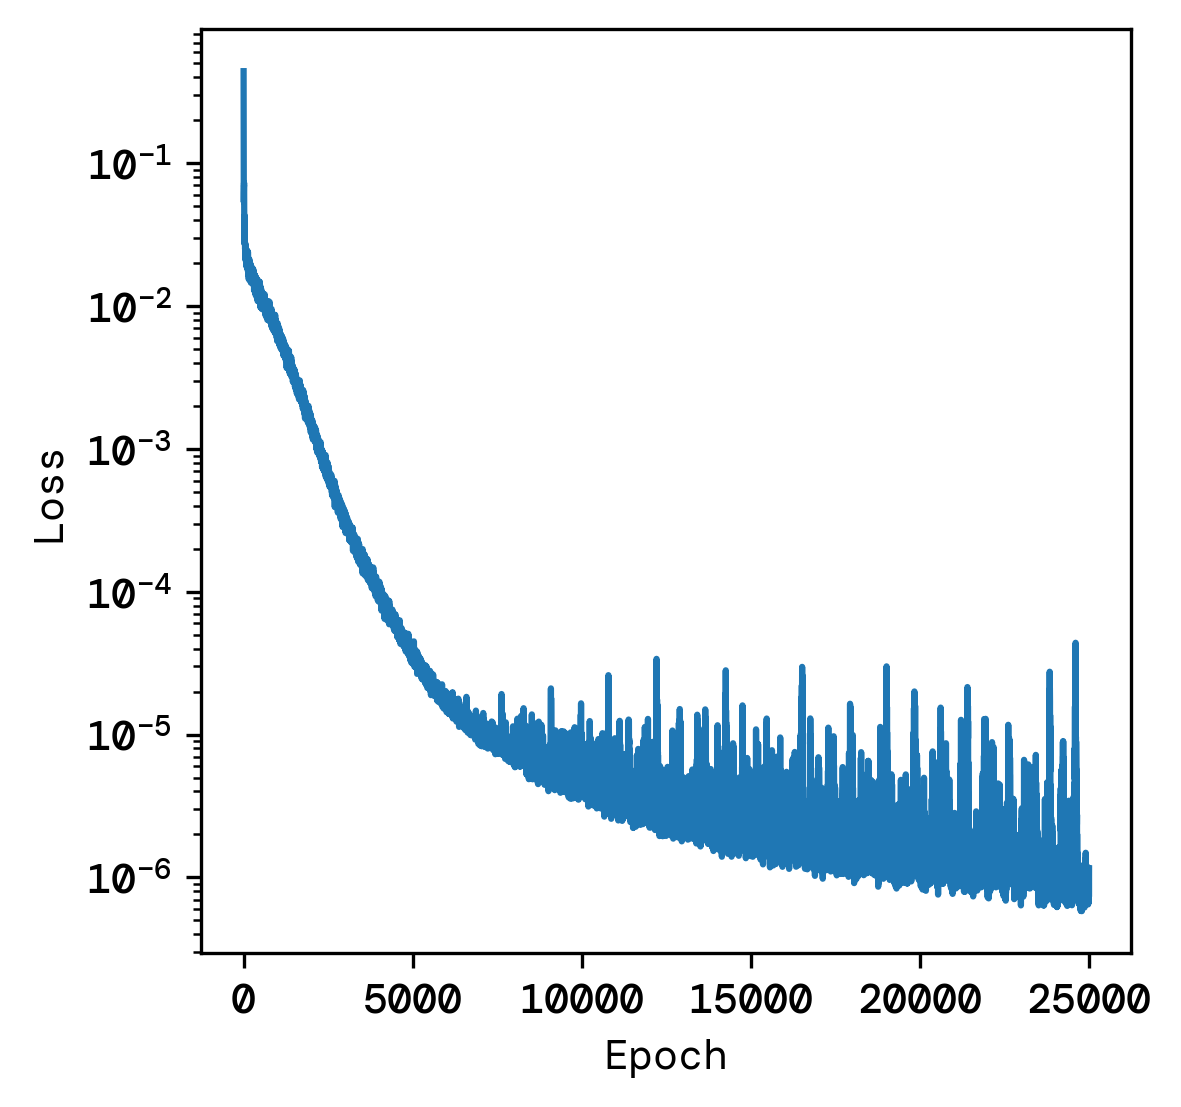
\includegraphics[width=\textwidth]{../runsAndFigures/wave_tf_hybrid_loss.png}
            \end{center}
            \caption
            {
                The PINN learns a solution to the wave equation where the initial momentum is not defined.
                Yet it satisfies the wave equation and the initial conditions.
            }\label{fig:wave_tf_dnn}
        \end{minipage}
    \end{figure}


    \begin{figure}[!ht]
        \begin{minipage}[t]{0.5\textwidth - 1mm}
            \begin{center}
                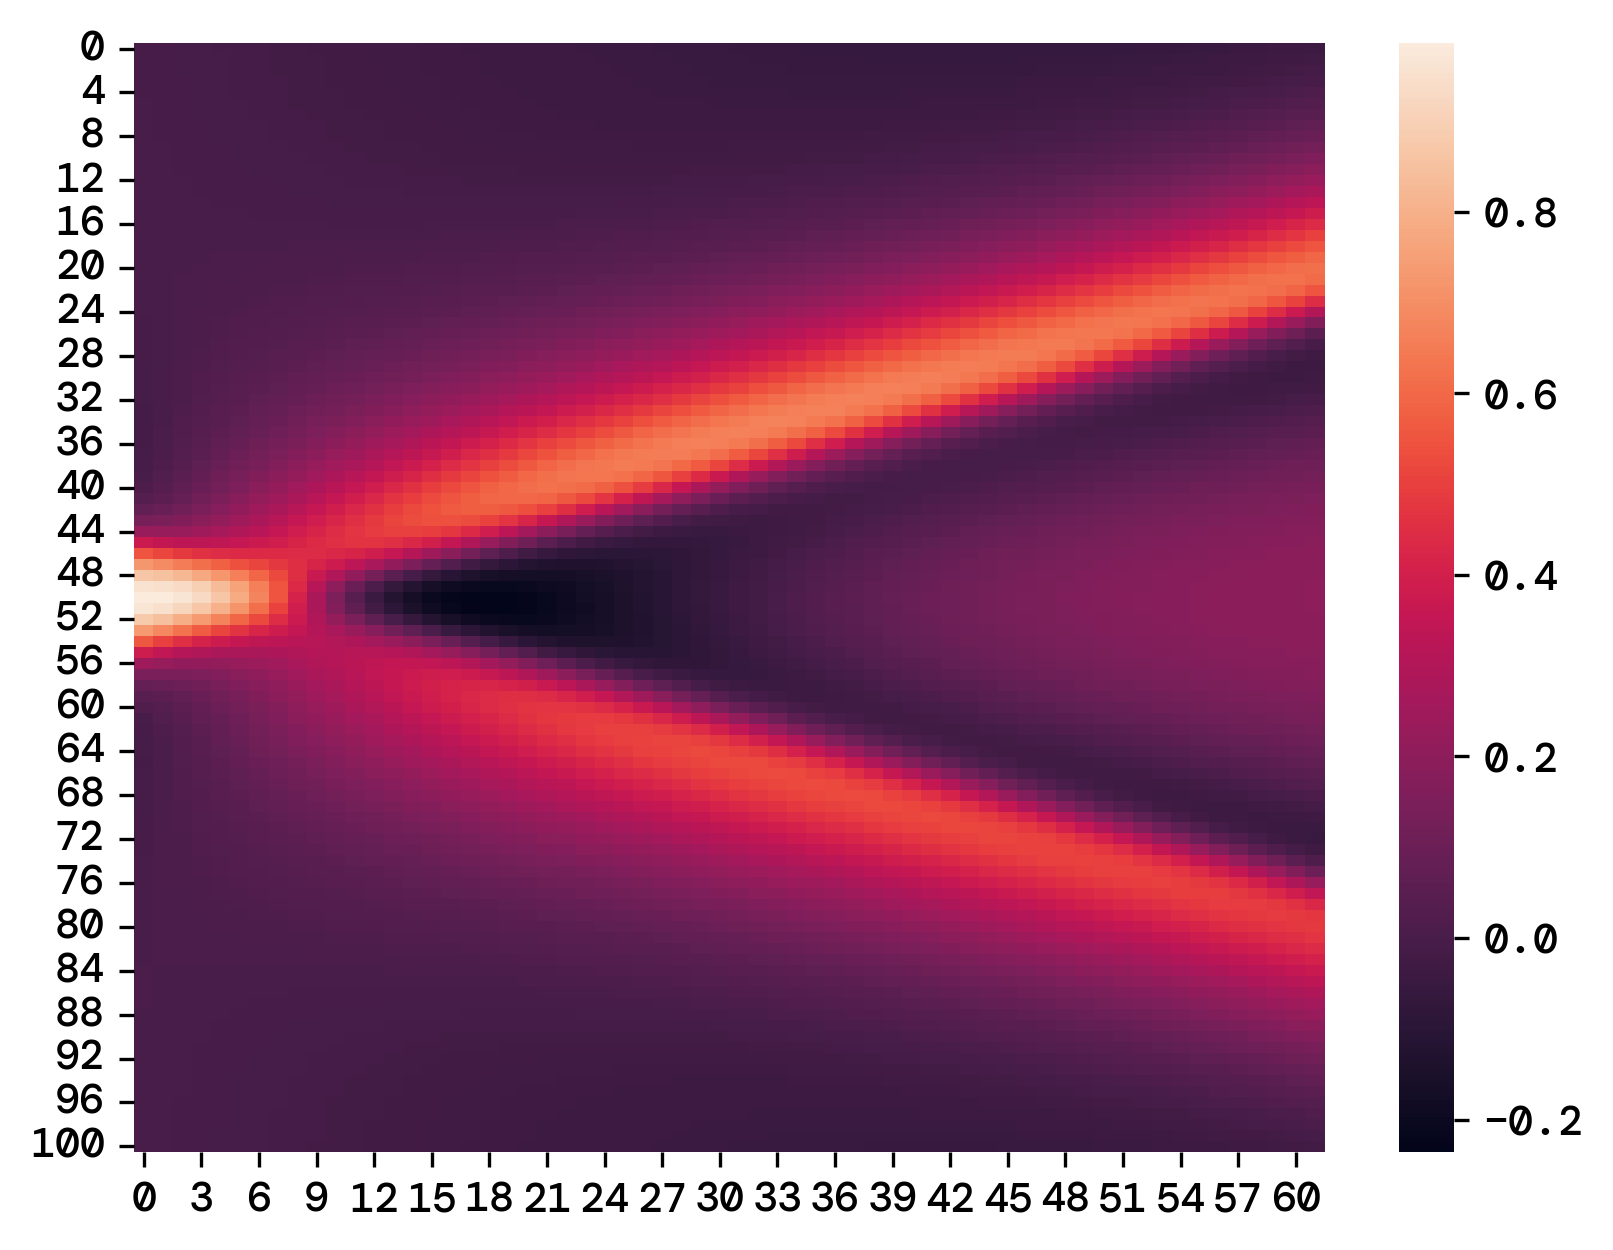
\includegraphics[width=\textwidth]{../runsAndFigures/wave_tf_pinn.png}
            \end{center}
            \caption
            {
                PINN solution to the wave equation.
            }\label{fig:wave_own_dnn}
        \end{minipage}
        \hspace{2mm}
        \begin{minipage}[t]{0.5\textwidth - 1mm}
            \begin{center}
                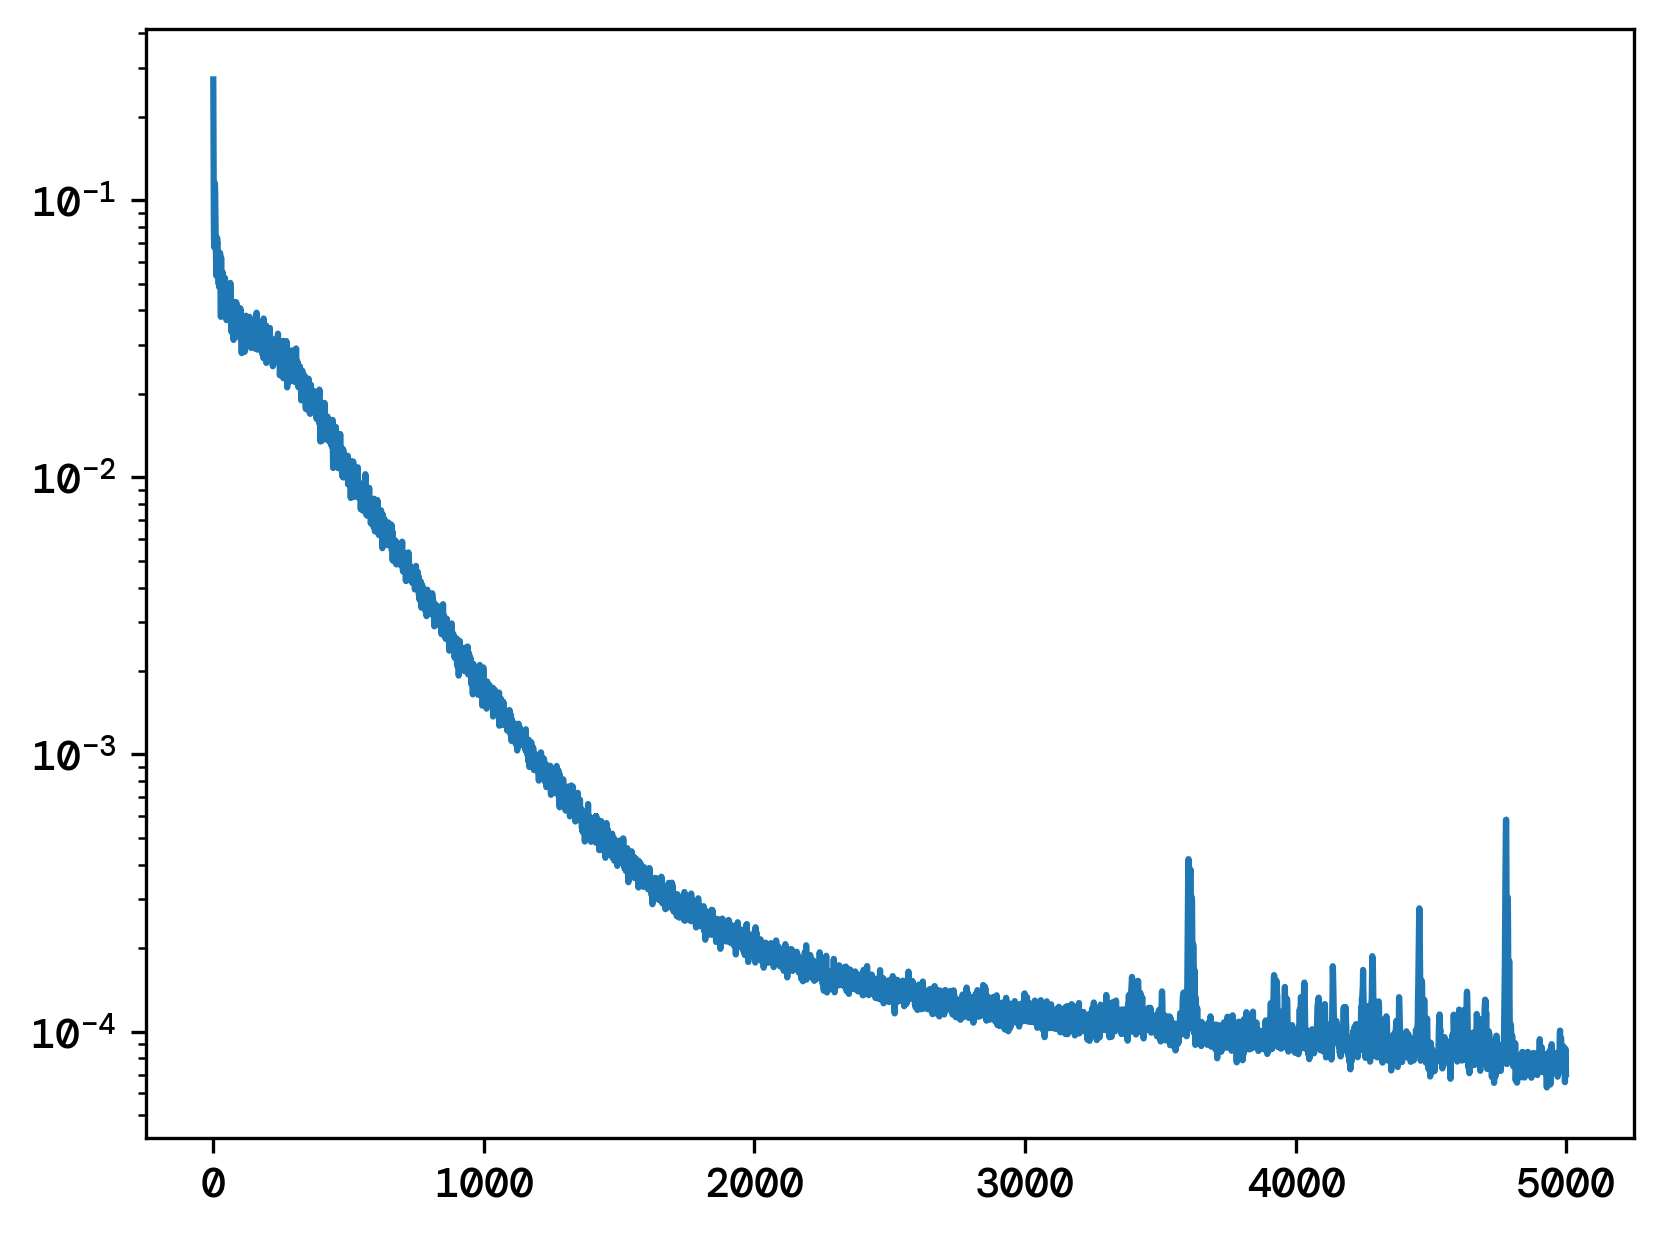
\includegraphics[width=\textwidth]{../runsAndFigures/wave_tf_pinn_loss.png}
            \end{center}
            \caption
            {
                The PINN learns a solution to the wave equation where the initial momentum is not defined.
                Yet it satisfies the wave equation and the initial conditions.
            }\label{fig:wave_tf_dnn}
        \end{minipage}
    \end{figure}

    \begin{figure}[!ht]
        \begin{minipage}[t]{0.5\textwidth - 1mm}
            \begin{center}
                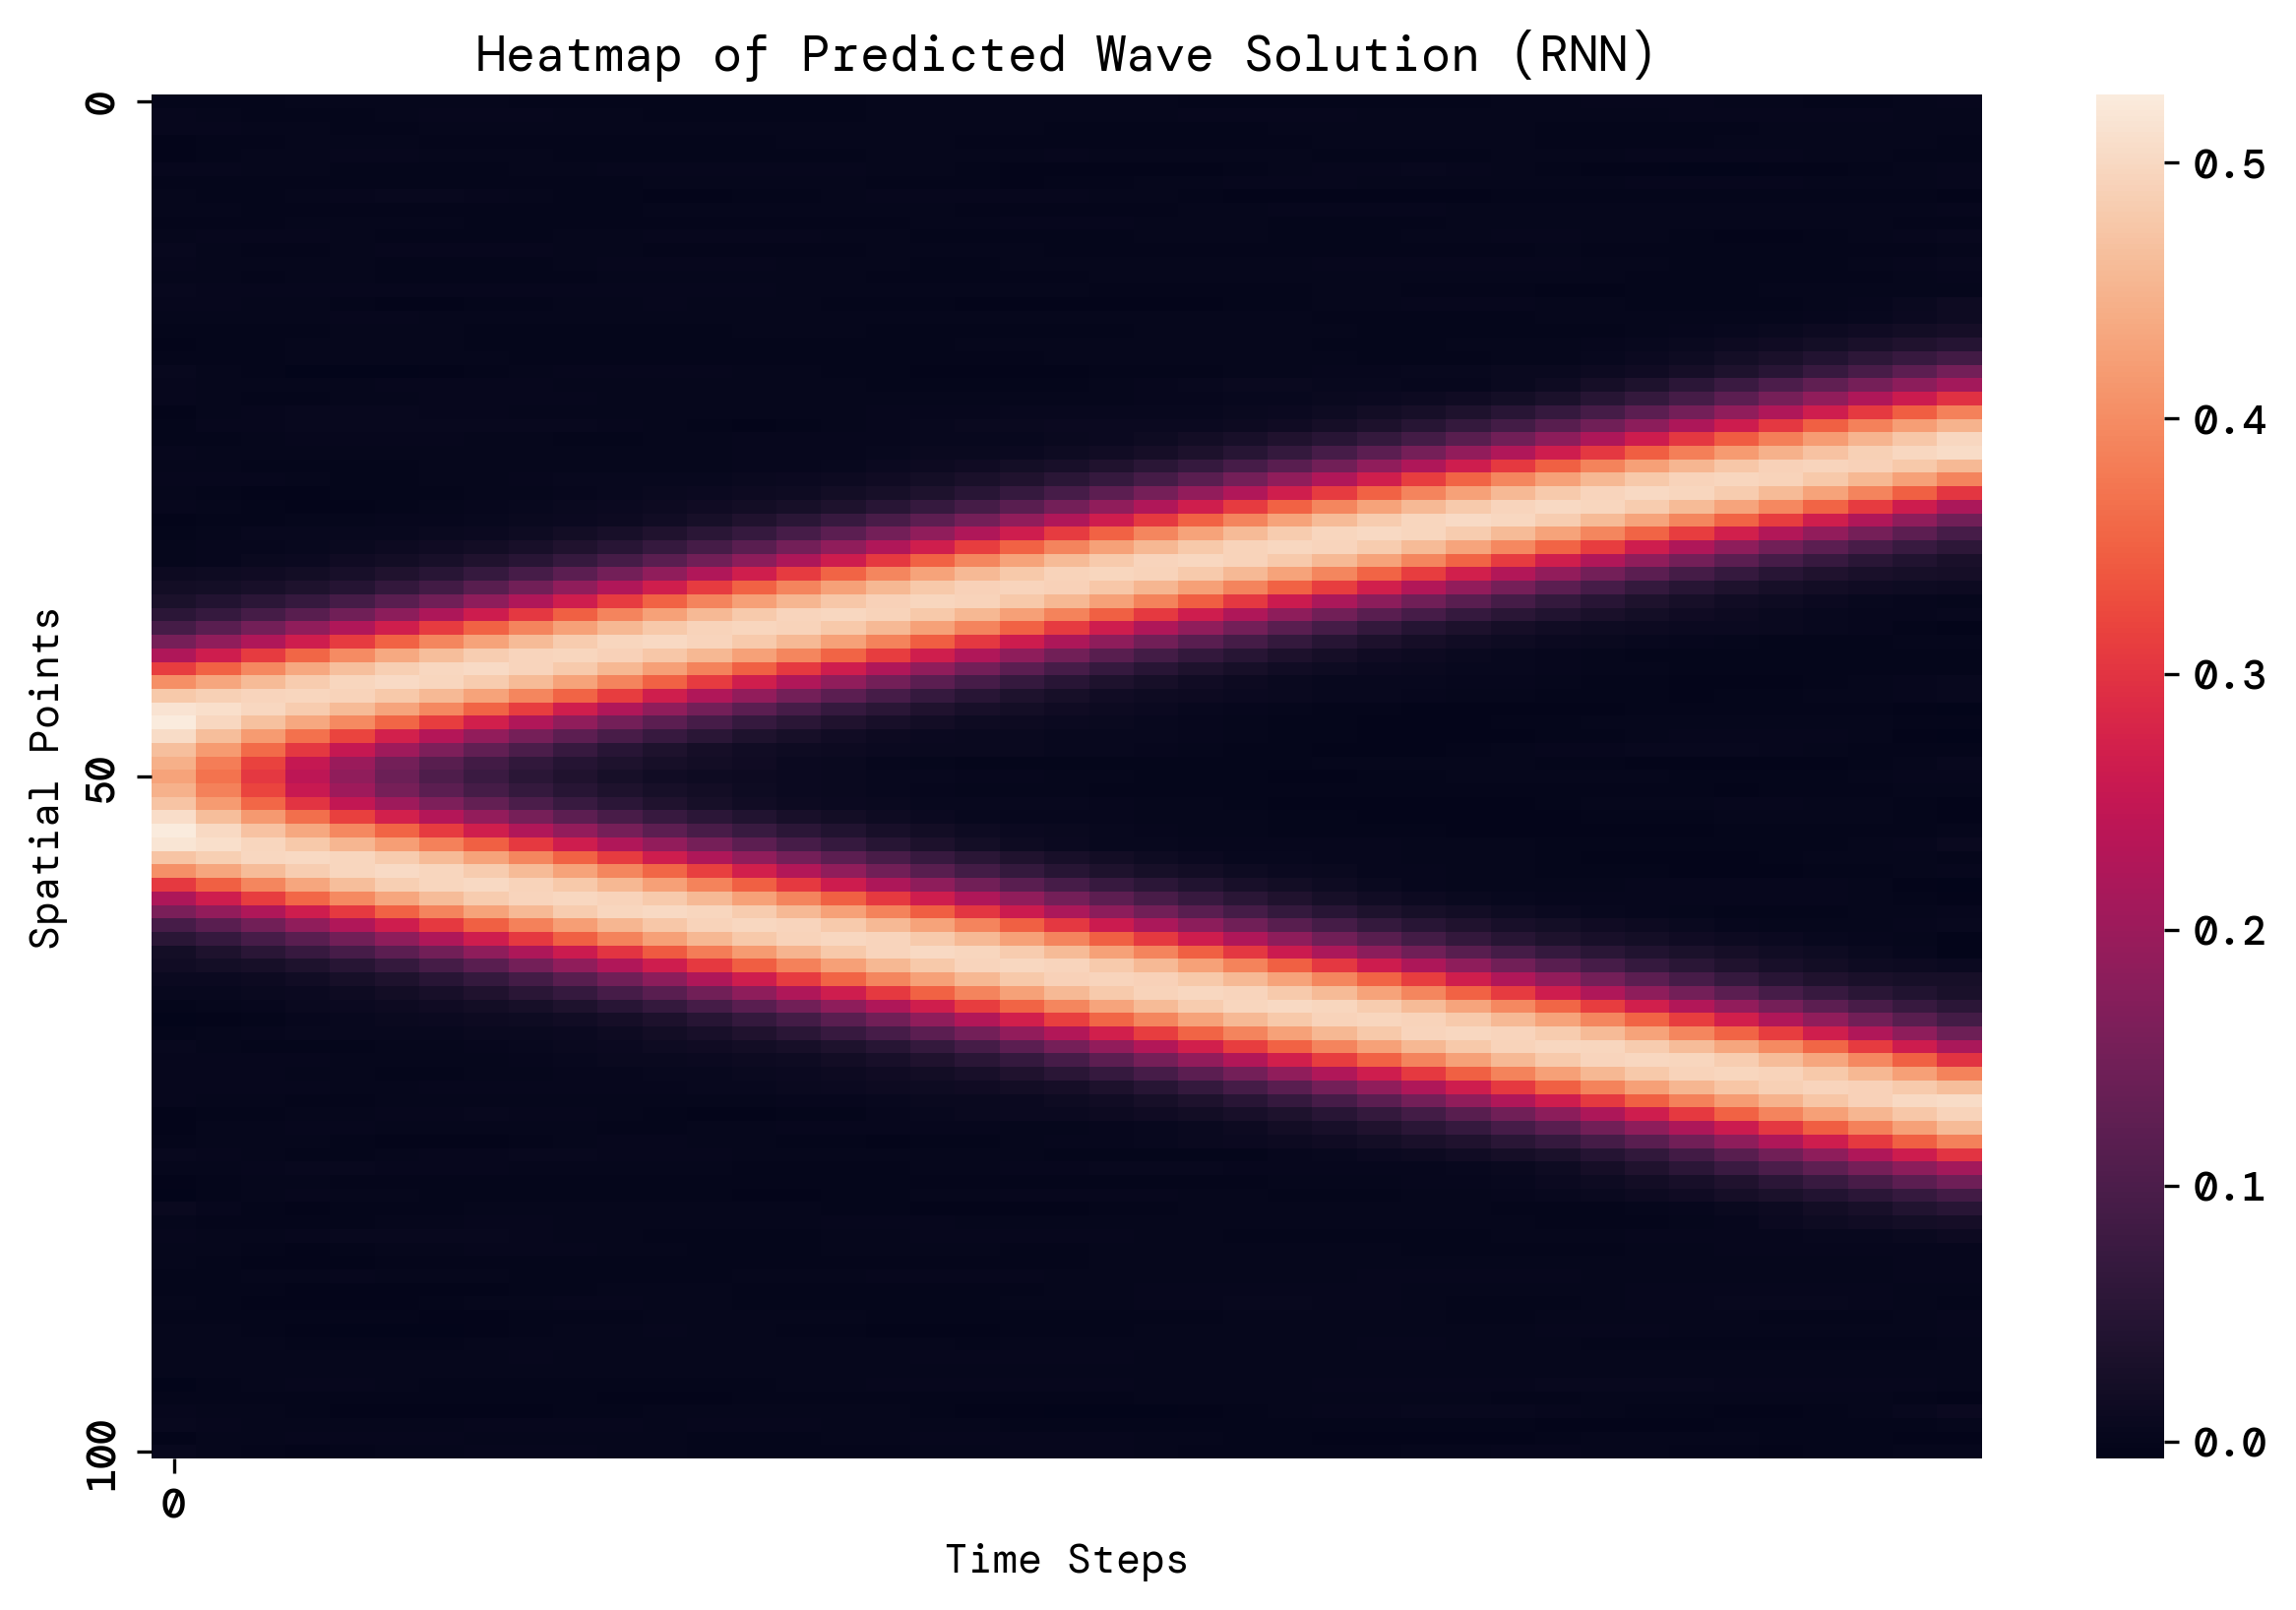
\includegraphics[width=\textwidth]{../runsAndFigures/wave_rnn.png}
            \end{center}
            \caption
            {
                PINN solution to the wave equation.
            }\label{fig:wave_own_dnn}
        \end{minipage}
        \hspace{2mm}
        \begin{minipage}[t]{0.5\textwidth - 1mm}
            \begin{center}
                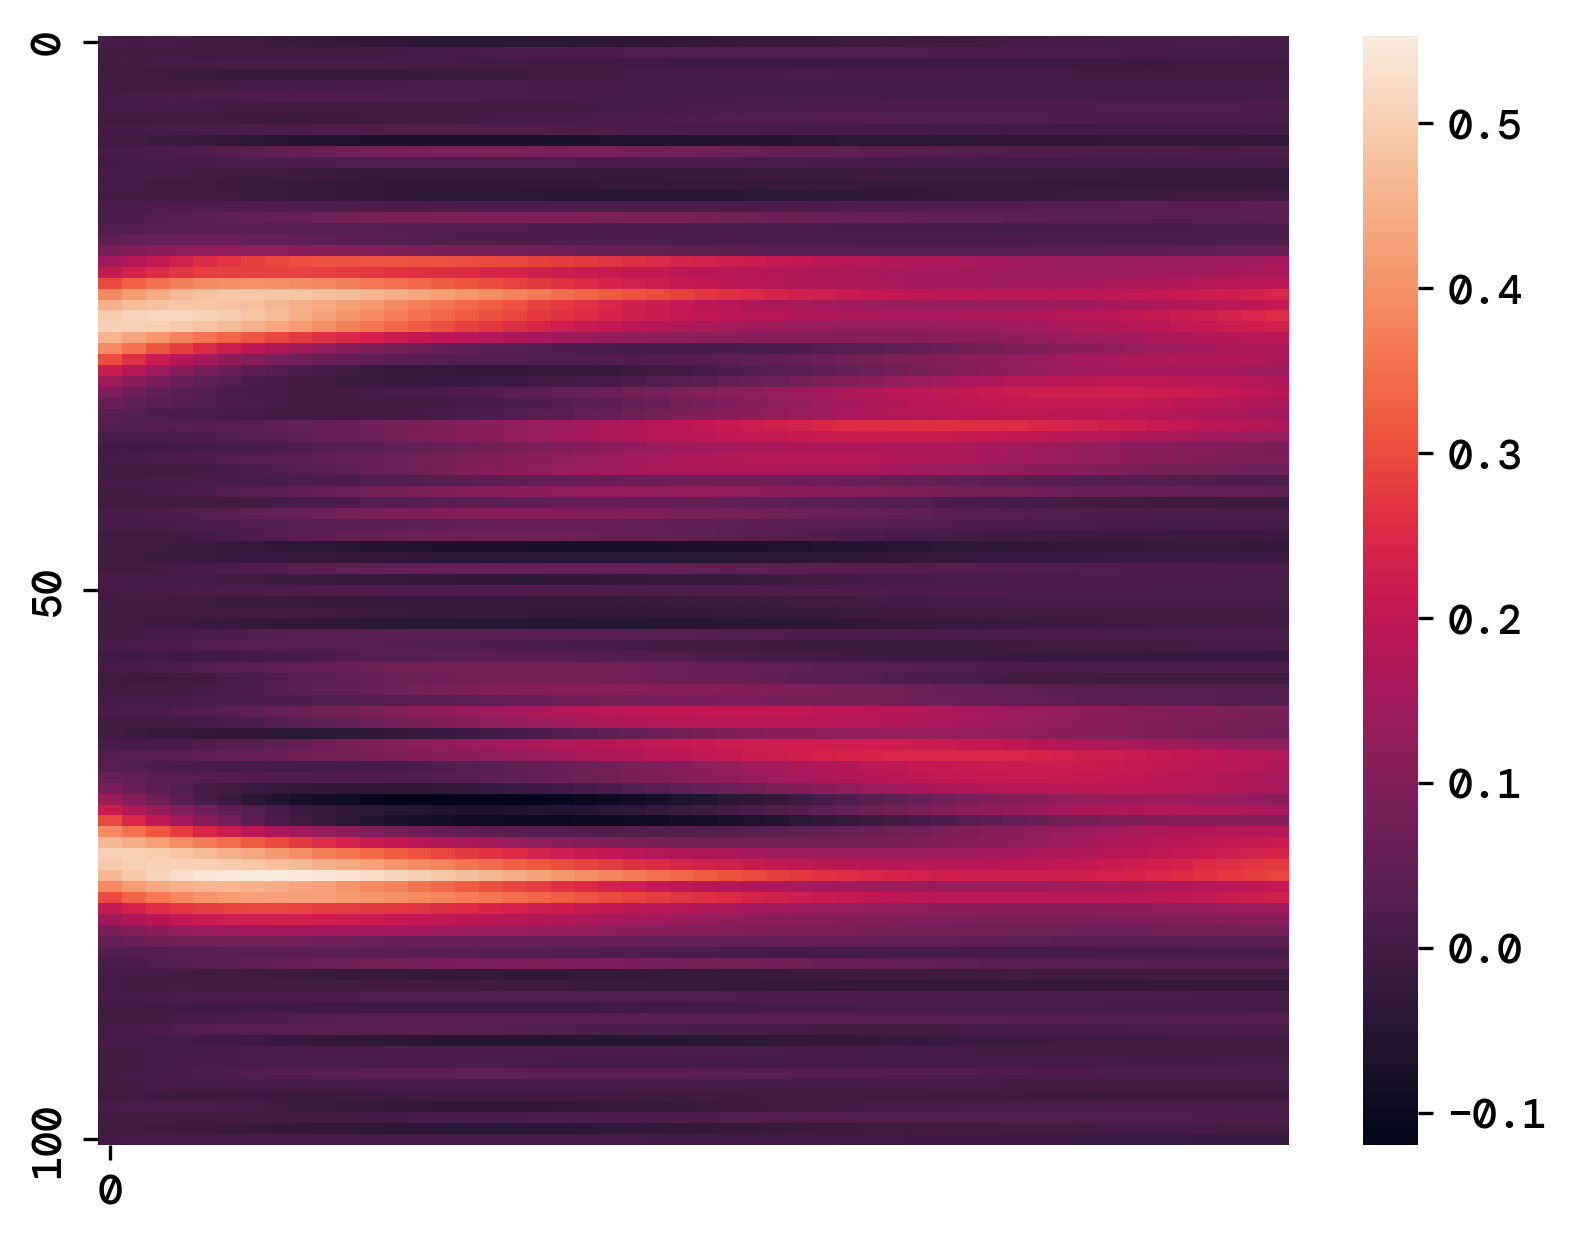
\includegraphics[width=\textwidth]{../runsAndFigures/wave_rnn_future.png}
            \end{center}
            \caption
            {
                The PINN learns a solution to the wave equation where the initial momentum is not defined.
                Yet it satisfies the wave equation and the initial conditions.
            }\label{fig:wave_tf_dnn}
        \end{minipage}
    \end{figure}

    We can see that the RNN strugles generate new data points. In fact for our case the PINN is far greater at this task.
    as we can train it on a small time frame and get good approximations for the rest of the time frame. We think 
    that the RNN would be better suited for problems where we want to generalize to other initial conditions,
    with more data available.


\subsection{Hyperparameters}
\label{sec:hyperparameters}

    As this is a proof of concept, we have not spent much time tuning hyperparameters. We have however
    done some experiments to get a feel for how the hyperparameters affect the performance of the models.
    We have also done some experiments to see how the different components of the loss function affect
    the performance of the hybrid solver. We have not done any experiments to see how the hyperparameters
    affect the performance of the RNN model, as this would require a lot of time and computational resources.

    We have however done some experiments to see how the different components of the loss function affect
    the performance of the RNN model.

    training time

    This paper shows that a carefully designed loss function goes a long way and many techniques can b combined trough
    the loss function. If we have some prior knowledge about the problem, we can bake this into the loss function.
    improving the model's performance.

\newpage
\subsection{Comparisons}
\label{sec:comparisons}




    
\section{Conclusion}
\label{sec:conclusion}

    We have explored the use of neural networks in solving the wave equation. Our findings indicate that
    neural networks are capable of approximating the wave equation, although the accuracy of the models
    is not as high as we would have hoped. For our simple case where both analytical and finite difference
    solutions are available, the neural network models are not able to achieve the same accuracy. 
    However, as the partial differential equations become
    more complex, the analytical solutions may be impossible to find, and the finite difference solutions
    may become too computationally expensive or inaccurate. In these cases, neural networks may be a
    viable alternative.
    Future work could involve exploring more complex partial differential equations , such as the
    Navier-Stokes equations, with more complex bounds and initial conditions 
    and comparing the accuracy of the neural network models to the analytical
    and finite difference solutions. Another interesting direction would be to explore the use of


    
    
     








% \acks{}


% \clearpage 
%
% \appendix
% \renewcommand{\theHchapter}{appendix\Alph{chapter}}
% \renewcommand{\theHsection}{appendix\thesection}
%
% \phantomsection
% \addcontentsline{toc}{chapter}{Appendix}
%
%
% \chapter*{Appendix A}
% \label{app:appendixA}




\vskip 0.2in
\bibliography{report}
\bibliographystyle{apalike}
% \bibliographystyle{plain}
\addcontentsline{toc}{section}{Bibliography}
\end{document}

